
%%%%%%%%%%%%%%%%%%%%%%%%%%%%%%%%%%%%%%
%
%     TITLE NAME
%
%%%%%%%%%%%%%%%%%%%%%%%%%%%%%%%%%%%%%%
%\href{https://www.home.me}{homepage.com}
\namesection{Yahya}{Shubbak}{M.Sc. Nanoscience, University of Kassel \hfill \today }{\contactline
{\href{https://github.com/YahyaShubbak}{NanoYahya}}{\href{https://www.linkedin.com/in/yahya-shubbak-75a537229/}{Yahya Shubbak}}{\href{mailto:y.shubbak@ik.me}{y.shubbak@ik.me}}{\href{tel:+4917680848963}{+49 17680848963}}}

% \namesection{Firstname}{Lastname}{Full Stack Software Engineer}{\contactline{\href{https://www.mazumder.me}{mazumder.me}}{\href{https://www.github.com/sansquoi}{sansquoi}}{\href{https://www.linkedin.com/mazumders}{mazumders}}{\href{mailto:shubham.mazumder@gmail.com}{first.last@email.com}}{\href{tel:+1999999999}{9999999999}}}

%%%%%%%%%%%%%%%%%%%%%%%%%%%%%%%%%%%%%%
%
%     COLUMN ONE
%
%%%%%%%%%%%%%%%%%%%%%%%%%%%%%%%%%%%%%%

%%%%%%%%%%%%%%%%%%%%%%%%%%%%%%%%%%%%%%
%     EXPERIENCE
%%%%%%%%%%%%%%%%%%%%%%%%%%%%%%%%%%%%%%

\sectionsep
\section{Experience}
\runsubsection{University Research and Teaching} \\
\location{June 2022 – today | 3 months | \color{UniKassel}  \textsc{University of Kassel}, Germany}
%\vspace{\topsep}
\begin{tightemize}
\item Research assistant in the group of Prof. Dr. Arno Ehresmann

Enhancing the experimental particle transport setup, utilizing the dark field capabilities of a new microscope
\end{tightemize}
\begin{tightemize}
\item Coordinator for the physics tutorial and exam for electrical engineering students

Design of the exercise sheets and exam, weekly briefing of the tutors to prepare them for the tutorial 
\end{tightemize}
\location{November 2021 – April 2022 | 6 months | \color{UniKassel}  \textsc{University of Kassel}, Germany }
%\vspace{\topsep}
\begin{tightemize}
\item Research assistant in the group of Prof. Dr. Arno Ehresmann

Working in the lab with magnetic thin films and -beads in preparation for the PhD position. Supervision of a research internship was among the responsibilities.
\end{tightemize}
\location{February 2020 – May 2020 | 4 months | \color{UV} \textsc{University of València}, Spain}
\begin{tightemize}
\item Research assistant in the group of Prof. Dr. Eugenio Coronado

Fabricating spin-crossover thin-film devices of different molecular systems for physical investigation   
\end{tightemize}
\location{May 2019 – August 2019 | 4 months  | \color{UniKassel}  \textsc{University of Kassel}, Germany}
\begin{tightemize}
\item Research assistant in the group of Prof. Dr. Arno Ehresmann

Using a self-designed fiber adaptation for a Czerny-Turner-spectrometer with a position sensitive detector, Carbon, Titan and Iron bands were spectroscopically analysed with the astrophysics group of Prof. Dr. Thomas Giesen
\end{tightemize}
\location{October 2018 - February 2019 | 5 months  | \color{UniKassel}  \textsc{University of Kassel}, Germany}
\begin{tightemize}
% \item Tutor for \emph{General Chemistry for Civil- and Enviromental Engineers}
\item Tutor for \begin{em}
General Chemistry for Civil- and Enviromental Engineers
\end{em}

Weekly in-person tutoring of the lecture on general chemistry in front of 40+ students.
\end{tightemize}

\sectionsep
\runsubsection{Research stay}\\
\location{April 2022 | Paris, France}
\begin{tightemize}
\item Beamtime at HERMES, Synchrotron facility Soleil, measurements for the Group of Ehresmann
\end{tightemize}
\location{September 2020 | Barcelona, Spain}
\begin{tightemize}
\item Beamtime at BOREAS, Synchrotron facility Alba, measurements for my masters thesis
\end{tightemize}

\sectionsep

\runsubsection{Conference Contributions} \\
\location{Fall 2022 | Regensburg, Germany}
\begin{tightemize}
\item DPG Congress of the Condensed Matter Section with a poster presentation, titled

\textit{X-Ray Characterization of an Above-RT bi-Stable Sublimable Molecular Spin-Crossover Fe(II)-Complex}



Largest physics congress in Europe with over 4000 visitors from 40 countries and 3600 contributions
\end{tightemize}
\location{Spring 2022 | Kassel, Germany}
\begin{tightemize}
\item 20 years CINSaT workshop with a poster presentation, titled

\textit{Above-RT bi-Stable Sublimable Molecular Spin-Crossover
Fe(II)-Complex – Concept and Characterization}
\end{tightemize}
\location{Fall 2021 | Kassel, Germany}
\begin{tightemize}
\item CINSaT Fall Colloquium with a poster presentation (from 84th DPG, due to the DPG held online) 
\end{tightemize}
\location{Fall 2021 | online}
\begin{tightemize}
\item 84th Annual Meeting of DPG of the Condensed Matter Section, poster presentation titled:

\textit{High throughput analysis of surface-functionalized superparamagnetic particles in dynamic magnetic field landscapes}
\end{tightemize}

\section{References} 
\href{http://ag-ehresmann.de/}{\textbf{Prof. Dr. Arno Ehresmann}, Professor, University of Kassel}


\begingroup
\setbox0=\hbox{

\includegraphics[scale=0.1,trim={0 1cm 0cm 0cm}]{icons/main/mail.png}\hspace{0.1cm}
\href{mailto:ehresmann@physik.uni-kassel.de}{ehresmann@physik.uni-kassel.de} 
}
\parbox{\wd0}{\box0}
\endgroup
\begingroup
\setbox0=\hbox{

\includegraphics[scale=0.1,trim={0 1.25cm -0.4cm 0cm}]{icons/main/phone.png}\hspace{0.1cm}+49 561 804-4060
}
\parbox{\wd0}{\box0}\endgroup
\\
\sectionsep
\href{https://www.linkedin.com/in/navarro-moratalla-efrén-1bb1b4a5/?originalSubdomain=es} {\textbf{Dr. Efrén Navarro Moratalla}, Research Fellow, Group Leader, University of València} 
\\
\begingroup
\setbox0=\hbox{

\includegraphics[scale=0.1,trim={0 1cm 0cm 0cm}]{icons/main/mail.png}\hspace{0.1cm}  	\href{mailto:efren.navarro@uv.es}{efren.navarro@uv.es}
}
\parbox{\wd0}{\box0}
\endgroup
\begingroup
\setbox0=\hbox{

\includegraphics[scale=0.1,trim={0 1.25cm -0.4cm 0cm}]{icons/main/phone.png}\hspace{0.1cm}+34 963544181
}
\parbox{\wd0}{\box0}\endgroup
\\
\sectionsep
\href{https://contacts.ucalgary.ca/info/phas/profiles/486-153949} {\textbf{Prof. Dr. Paul Barclay}, Professor, University of Calgary} 
\\
\begingroup
\setbox0=\hbox{

\includegraphics[scale=0.1,trim={0 1cm 0cm 0cm}]{icons/main/mail.png}\hspace{0.1cm}  	\href{mailto:pbarclay@ucalgary.ca}{pbarclay@ucalgary.ca}
}
\parbox{\wd0}{\box0}
\endgroup
\begingroup
\setbox0=\hbox{

\includegraphics[scale=0.1,trim={0 1.25cm -0.4cm 0cm}]{icons/main/phone.png}\hspace{0.1cm}+1 403 220-8517
}
\parbox{\wd0}{\box0}\endgroup
\\
%\href{https://contacts.ucalgary.ca/info/phas/profiles/1-6248004} %{\textbf{Dr. Sean Stotyn}, Associate Professor, University of Calgary} 
%\\
%\begingroup
%\setbox0=\hbox{
%
\includegraphics[scale=0.1,trim={0 1cm 0cm %0cm}]{icons/main/mail.png}\hspace{0.1cm}  	%\href{mailto:sean.stotyn@ucalgary.ca}{sean.stotyn@ucalgary.ca}
%}
%\parbox{\wd0}{\box0}
%\endgroup
%\begingroup
%\setbox0=\hbox{
%
\includegraphics[scale=0.1,trim={0 1.25cm -0.4cm %0cm}]{icons/main/phone.png}\hspace{0.1cm}+1 403 210-7594
%}
%\parbox{\wd0}{\box0}\endgroup
%\\



\newpage
\section{Awards}

\runsubsection{Scholarship} \\
%\descript{| Studienstiftung des deutschen Volkes}
\location{September 2017 | 3 weeks | \color{StuStiOrange}\textsc{Studienstiftung des deutschen Volkes}}
\begin{tightemize}
\item Fully funded language fellowship in La Rochelle, France, to learn French.
\end{tightemize}
\location{August 2016 - March 2017 | 8 months | \color{StuStiOrange}\textsc{Studienstiftung des deutschen Volkes}}
\begin{tightemize}
\item Fully-funded scholarship to study at the University of Calgary, Canada, including tuition fees and living expenses %for two terms
\end{tightemize}
\location{April 2015 - September 2017 | 2 years, 6 months | \color{StuStiOrange}\textsc{Studienstiftung des deutschen Volkes}}
\begin{tightemize}
\item The German National Academic Foundation (Studienstiftung des deutschen Volkes) awards full scholarships to outstanding German undergraduate and graduate students. Scholarships are based on academic excellence and awarded to less than 
0.5\hspace{0.7pt}\%
of students studying all subjects nationwide in Germany. The Studienstiftung promotes future excellence in the areas of science, business, public administration, and the arts.
\end{tightemize}





\section{Education}
\runsubsection{Doctorate Research}
%\descript{| University of Kassel} 
\\
\location{June 2022 – today | \color{UniKassel}  \textsc{University of Kassel}, Germany}
\vspace{\topsep} % Hacky fix for awkward extra vertical space
\begin{tightemize}
%\sectionsep
\item Research topic: 

\textit{Harnessing close-to-surface transport of magnetic particles in a dynamically transformed magnetic field landscapes for Lab-on-a-chip applications}
\end{tightemize}

\sectionsep

\runsubsection{Master of Science}
%\descript{| University of Kassel \& University of València}
\\
\location{April 2019 – March 2022 | \color{UniKassel}  \textsc{University of Kassel}, Germany \color{black} \& \color{UV} \textsc{University of València}, Spain}
%\vspace{\topsep} % Hacky fix for awkward extra vertical space
\begin{tightemize}
%\sectionsep
\item Master thesis in nanoscience at the department of atomic and molecular physic, titled 

\textit{Processing and Characterization of a bi-Stable Sublimable Molecular Spin-Crossover Fe(II)-Complex}

Graded \textbf{1.15} (excellent). Cumulative grade: \textbf{1.3} (very good)
\end{tightemize}

\location{September 2019 - October 2020 | \color{UV} \textsc{University of València}, Spain}
%\vspace{\topsep} % Hacky fix for awkward extra vertical space
\begin{tightemize}
\item Erasmus at the University of València in the master program \textit{Molecular Nanocience and Nanotechnology} combined with the research for the master thesis
\end{tightemize}

\sectionsep

\runsubsection{Bachelor of Science}
%\descript{| University of Kassel}
\\
\location{October 2014 – June 2019 | \color{UniKassel}  \textsc{University of Kassel}, Germany}
%\vspace{\topsep} % Hacky fix for awkward extra vertical space
\begin{tightemize}
%\sectionsep
\item Bachelor thesis in nanoscience at the department of atomic and molecular physic, titled 

\textit{Design and Characterization of a Fiber Adaptation for a Czerny-Turner-Spectrometer with a Position sensitive Detector at the Example of Carbon Emission Lines - Swan Bands} 

Graded \textbf{1.86} (very good). Cumulative grade: \textbf{2.2} (good)
\end{tightemize}

\location{September 2016 - May 2017 | \color{UniCalgary} \textsc{University of Calgary}, Canada}
%\vspace{\topsep} % Hacky fix for awkward extra vertical space
\begin{tightemize}
\item Studies abroad at the University of Calgary at the Physics department
\end{tightemize}
\sectionsep

\runsubsection{School Education}
%\descript{| Kassel } 
\\
%\location{September 2011 – July 2014 | High School | Elisabeth-Knipping-Schule Kassel | Abitur 1.8 }
%\location{September 2005 – July 2011 | Middle School | Gesamtschule Fuldatal}
%\location{August 2001 - July 2005 | Elementary School | Wolfsanger/Hasenhecke}
\location{August 2001 – July 2014 | Kassel, Germany }
\begin{tightemize}
\item Abitur (High School Diploma) at the Elisabeth-Knipping-Schule Kassel. 

Cumulative grade: \textbf{1.8} (very good)
\end{tightemize}

\begin{comment}

%%%%%%%%%%%%%%%%%%%%%%%%%%%%%%%%%%%%%%
%     Projects
%%%%%%%%%%%%%%%%%%%%%%%%%%%%%%%%%%%%%%

%\section{Awards}

%\runsubsection{Scholarship}
%\descript{| Studienstiftung des deutschen Volkes}
%\location{April 2015 - September 2017 | 2 years 6 months}
%\sectionsep

\section{Experience}
\runsubsection{University Research and Teaching} \\
%\descript{| University of Kassel}
\location{November 2021 – April 2022 | 6 months }
\begin{tightemize}
\item Research assistant in the group of Prof. Dr. Arno Ehresmann, University of Kassel \end{tightemize}
\location{February 2020 – May 2020 | 4 months}
\begin{tightemize}
\item Research assistant in the group of Prof. Dr. Eugenio Coronado, University of València 
\end{tightemize}
\location{May 2019 – August 2019 | 4 months}
\begin{tightemize}
\item Research assistant in the group of Prof. Dr. Arno Ehresmann, University of Kassel
\end{tightemize}
\location{October 2018 - February 2019 | 5 months}
\begin{tightemize}
\item Tutor "General Chemistry for Civil- and Enviromental Engineers", University of Kassel
\end{tightemize}
\vspace{\topsep} % Hacky fix for awkward extra vertical space
%\sectionsep
\runsubsection{Research stay}\\
\location{April 2022 | Paris, France}
\begin{tightemize}
\item Beam time at HERMES, Synchrotron facility Soleil
\end{tightemize}
\location{September 2020 | Barcelona, Spain}
\begin{tightemize}
\item Beam time at BOREAS, Synchrotron facility Alba
\end{tightemize}

\runsubsection{Conferences} \\
%\location{Fall 2022}
%\begin{tightemize}
%\item DPG Congress of the Condensed Matter Section in Regensburg, Germany, poster presentation 
%\end{tightemize}
\location{Spring 2022}
\begin{tightemize}
\item 20 years CINSaT workshop in Kassel, Germany, poster presentation 
\end{tightemize}
\location{Fall 2021}
\begin{tightemize}
\item CINSaT Fall Colloquium in Kassel, Germany, poster presentation 
\end{tightemize}
\location{Fall 2021}
\begin{tightemize}
\item 84th Annual Meeting of DPG of the Condensed Matter Section, poster presentation
\end{tightemize}
%%%%%%%%%%%%%%%%%%%%%%%%%%%%%%%%%%%%%%
%     AWARDS
%%%%%%%%%%%%%%%%%%%%%%%%%%%%%%%%%%%%%%

% \section{Awards} 
% \begin{tabular}{rll}
% 2020	     & Finalist & Lorem Ipsum\\
% 2018	     & $2^{nd}$ & Dolor Sit Amet\\
% 2015	     & Finalist  & Cras posuere\\
% \\
% \end{tabular}
% \sectionsep
%%%%%%%%%%%%%%%%%%%%%%%%%%%%%%%%%%%%%%
%
%     COLUMN TWO
%
%%%%%%%%%%%%%%%%%%%%%%%%%%%%%%%%%%%%%%
\end{comment}


%%%%%%%%%%%%%%%%%%%%%%%%%%%%%%%%%%%%%%
%     SKILLS
%%%%%%%%%%%%%%%%%%%%%%%%%%%%%%%%%%%%%%
%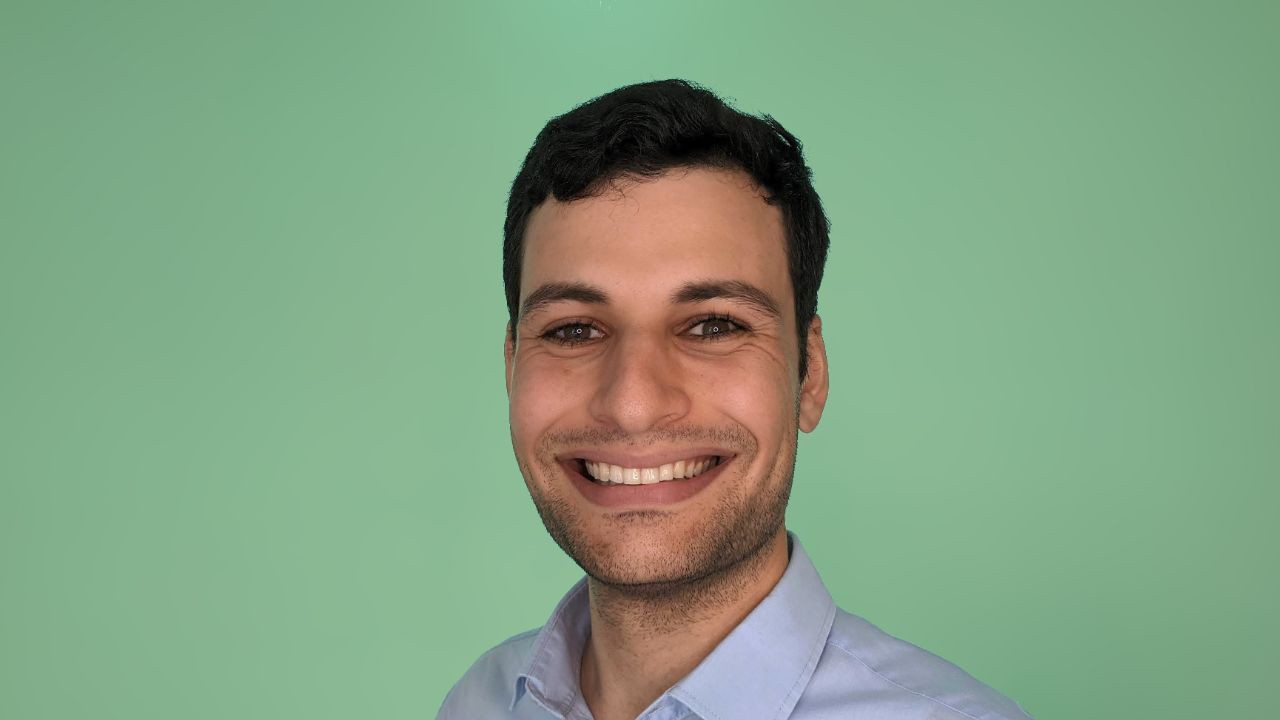
\includegraphics[width=0.8\linewidth,trim={12cm 0 8cm 1cm},clip]{icons/Yahya.jpg}



\begin{minipage}[t]{0.63\textwidth}
\section{Outreach}
\subsection{Voluntary Work} 
\location{October 2013 - July 2014 | \color{black}\textsc{Elisabeth-Knipping-Schule}, Kassel}
\vspace{\topsep}
\begin{tightemize}
\item School representative for over 2400 pupils
\end{tightemize}
\location{September 2008 - July 2010 | \color{black}\textsc{Gesamtschule Fuldatal}, Kassel}
\begin{tightemize}
\item School representative for over 600 pupils  
\item  Member of the State Student Council
\end{tightemize}
\location{March 2008 - July 2010 |\color{black} \textsc{Jugend-Bildungswerk}, Kassel}
\begin{tightemize}
\item Young Member of the Technical Committee (organizing seminars)
\end{tightemize}
\location{February 2007 - July 2010 | \color{black}\textsc{Gesamtschule Fuldatal}, Kassel}
\begin{tightemize}
\item Student mediator, helping about 2-6 pupils per week, including training for other mediators and helping in a seminar
\end{tightemize}
\end{minipage}
\begin{minipage}[t]{0.15\textwidth}

\section{Skills}

\subsection{Languages}
%\sectionsep
\location{Mother Tongues:}
Arabic \textbullet{} German \\
%\sectionsep
\location{C1 ILETS Certificate:}
English \\
\sectionsep
\location{B1 Level:}
Spanish \\
\location{A1 Level:}
French \\
\end{minipage}
%\begin{minipage}[t]{0.17\textwidth}
%\section{}
%\subsection{Programming}
%\sectionsep
%\location{Intermediate:}
%Python \end{minipage}
\begin{minipage}[t]{0.2\textwidth}
\section{}
\subsection{Programming}
%\sectionsep
\location{Intermediate:}
Python
\subsection{Markup language}
\location{Advanced:}
\LaTeX
\subsection{Software}
%\sectionsep
\location{Advanced:}
Adobe Lightroom, Inkscape, Jabref,  Microsoft Office \\
\sectionsep
\location{Intermediate:}
Autodesk Inventor, Citavi\\\end{minipage}


% %%%%%%%%%%%%%%%%%%%%%%%%%%%%%%%%%%%%%%
% %     REFERENCES
% %%%%%%%%%%%%%%%%%%%%%%%%%%%%%%%%%%%%%%



%%%%%%%%%%%%%%%%%%%%%%%%%%%%%%%%%%%%%%
%     COURSEWORK
%%%%%%%%%%%%%%%%%%%%%%%%%%%%%%%%%%%%%%

% \section{Coursework}

% \subsection{Graduate}
% Graduate Algorithms \textbullet{}\\ 
% Advanced Computer Architecture \textbullet{}\\ 
% Operating Systems \textbullet{}\\ 
% Artificial Intelligence \textbullet{}\\
% Visualization For Scientific Data \\
% \sectionsep

% \subsection{Undergraduate}

% Database Management Systems \textbullet{}\\
% Object Oriented Analysis and Design \textbullet{}\\
% Artificial Intelligence and Expert Systems \textbullet{}\\
% Scripting Languages and Web Tech \textbullet{}\\
% Software Engineering \\



%%%%%%%%%%%%%%%%%%%%%%%%%%%%%%%%%%%%%%
%     Projects
%%%%%%%%%%%%%%%%%%%%%%%%%%%%%%%%%%%%%%

%\section{Awards}

%\runsubsection{Scholarship}
%\descript{| Studienstiftung des deutschen Volkes}
%\location{April 2015 - September 2017 | 2 years 6 months}
%\sectionsep


\vspace{\topsep} % Hacky fix for awkward extra vertical space
%\sectionsep

